\usetikzlibrary{positioning,calc,external,arrows.meta}

\title{ICS0026 Cryptography}
\subtitle{What's to come: post-quantum cryptography}
\date{\today}
\author{Taaniel Kraavi}
\institute%
{%
  \textit{IT College}\\
  \textit{Tallinn University of Technology}
}

\begin{document}
\begin{frame}
  \titlepage
\end{frame}

\begin{frame}{Classical cryptography}
  Common computational hardness assumptions for \enquote{classical} computers:
  \begin{itemize}[<+(1)->]
    \item Integer factorisation
    \item Discrete logarithm problem (DLP)
  \end{itemize}

  \vspace*{1em}

  \pause
  These problems are \enquote{easy} (crypto relevant) for quantum computers.
  \begin{itemize}[<+(1)->]
    \item Post-quantum cryptography (PQC)
    \item Shor's algorithm for integer factorisation
    \begin{itemize}
      \item There is a variant for solving the DLP
    \end{itemize}
    \item We need trapdoors not breakable by Shor's algorithm
    \begin{itemize}
      \item Algorithms should remain computable on classical computers
    \end{itemize}
  \end{itemize}
\end{frame}

\begin{frame}{Quantum computing}
  Quantum computing is done on quantum computers.
  \begin{itemize}[<+(1)->]
    \item Quantum bits called \emph{qubits}
    \item Quantum superposition of qubits
    \item More states than 0 or 1: probabilities of being either
    \item Computations in multiple \enquote{dimensions}: \enquote{parallelism}
    \item Currently they are not very reliable (physical vs logical qubit)
  \end{itemize}
\end{frame}

\begin{frame}{Quantum is picky}
  Currently there are no general purpose QC programming languages.
    \begin{itemize}[<+(1)->]
      \item Algorithms and programs must be carefully constructed
      \item Measurement performed at the end of the circuit (the \enquote{answer})
      \item If you measure a qubit directly, its state collapses: either 0 or 1
      \item Incorrect computation paths cancel out (destructive interference)
    \end{itemize}
\end{frame}

\begin{frame}{Dangerous algorithms}
  Shor's algorithm
  \begin{itemize}[<+(1)->]
    \item Integer factorisation
    \begin{itemize}
      \item Breaks RSA
    \end{itemize}
    \item Solving the DLP
    \begin{itemize}
      \item Breaks Diffie-Hellman (DH), elliptic-curve cryptography (ECC), \dots
    \end{itemize}
  \end{itemize}

  \pause

  Grover's algorithm
  \begin{itemize}[<+(1)->]
    \item Search algorithm
    \item Can be used for brute forcing: $O(N)_\mathit{classical} \to O(\sqrt{N})_\mathit{quantum}$
    \begin{itemize}
      \item 256 bits of classical security provide 128 bits of PQ security
      \item Argued to be an overly conservative estimate
      \item Symmetric crypto should remain safe for doubled security levels
    \end{itemize}
  \end{itemize}
\end{frame}

\begin{frame}{Post-quantum approaches}
  \begin{itemize}[<+(1)->]
    \item \enquote{symmetric} primitives
    \begin{itemize}
      \item no public-private correlation, just brute force
      \item symmetric encryption schemes (e.g. AES)
      \item hash-based cryptography (e.g. signatures)
      \item double the lengths due to Grover's algorithm since $\lambda_\mathit{classical} \to (\lambda/2)_\mathit{quantum}$
    \end{itemize}
    \item lattices
    \item isogenies of elliptic curves
    \item error-correcting codes
    \item multivariate polynomials
  \end{itemize}

  \vspace*{1em}

  \pause
  Lattice-based crypto seems to be the most popular PQC approach.
\end{frame}

\begin{frame}{Name-dropping lattices}
  \pause
  A lattice is an infinite grid of points.

  \vspace*{1em}

  \pause
  \begin{figure}
    \centering
    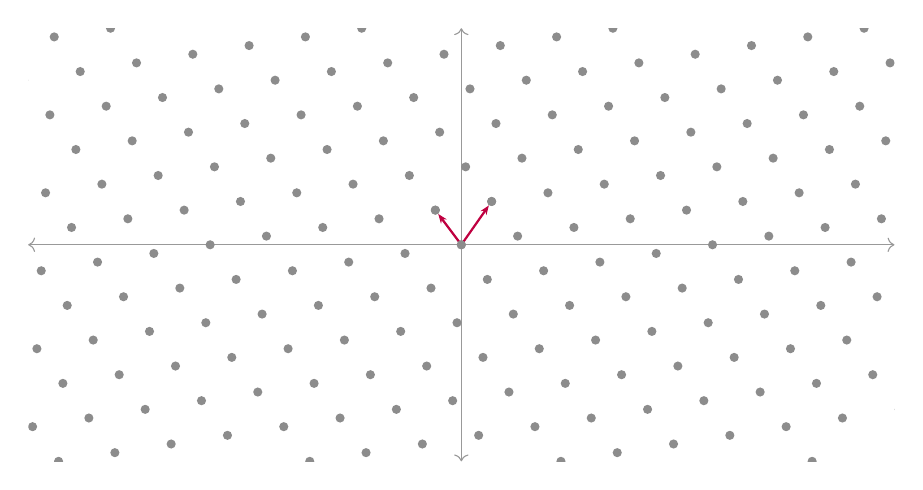
\begin{tikzpicture}
      \begin{scope}[scale=.55]
            \coordinate (Origin)   at (0,0);
            \coordinate (XAxisMin) at (-10,0);
            \coordinate (XAxisMax) at (10,0);
            \coordinate (YAxisMin) at (0,-5);
            \coordinate (YAxisMax) at (0,5);
            \draw [thin, black!40, <->] (XAxisMin) -- (XAxisMax);% Draw x axis
            \draw [thin, black!40,<->] (YAxisMin) -- (YAxisMax);% Draw y axis
            %\draw[style=help lines,dashed,black!20] (-5,-5) grid[step=1cm] (5,5);
    
            \begin{scope}
                \clip (-10,-5) rectangle (10,5); % Clips the picture...
                \pgftransformcm{1}{0.6}{0.7}{1}{\pgfpoint{0cm}{0cm}}
    
                % setup the nodes
                \foreach \x in {-20,...,20}
                \foreach \y in {-20,...,20}
                {
                  \node[shape=circle,fill=black!45,scale=0.35] (\x-\y) at (2*\x,\y+3){};
                }
            \end{scope}
    
            \node[shape=circle,fill=black!45,scale=0.35] (b1) at (-.6,.8){};
            \node[shape=circle,fill=black!45,scale=0.35] (b2) at (.7,1){};
            \draw [thick,purple,-{Stealth[length=1.2mm]}] (0,0) -- (b1);
            \draw [thick,purple,-{Stealth[length=1.2mm]}] (0,0) -- (b2);
            \node[shape=circle,fill=black!45,scale=0.35] at (0,0){};
    
        \end{scope}
    
      \end{tikzpicture}
  \end{figure}
\end{frame}

\begin{frame}{Name-dropping lattice problems}
  Some hard problems based on lattices:
  \begin{itemize}[<+(1)->]
    \item Shortest vector problem
    \begin{itemize}
      \item Find the shortest non-zero vector
    \end{itemize}
    \item Closest vector problem
    \begin{itemize}
      \item Find a vector closest to a given vector
    \end{itemize}
    \item Shortest independent vectors problem
    \begin{itemize}
      \item Find a basis with the shortest vectors
    \end{itemize}
  \end{itemize}

  \pause
  Solving one solves the others
  \begin{itemize}[<+(1)->]
    \item Crypto usually does not use them directly
    \item The other problems are then shown to be equivalent in difficulty
  \end{itemize}
\end{frame}

\begin{frame}{Name-dropping LWE}
  Learning with errors (LWE):
  \begin{itemize}[<+(1)->]
    \item Consider the linear equation system
    \[
      A \cdot s = b
    \]
    with $A \in \ZZ_q^{n \times m}$, $s\in\ZZ_q^m$, $b\in\ZZ_q^n$
    \item Add an error term $e\in\ZZ_q^n$ to obtain
    \[
      A \cdot s + e = b
    \]
    \item $s, e$ are secret, $A, b$ are public
    \item Variants exist: Ring-LWE, Module-LWE
  \end{itemize}
\end{frame}

\begin{frame}{NIST's PQC}
  \pause
  Key encapsulation mechanism (KEM)
  \begin{itemize}[<+(1)->]
    \item ML-KEM in \href{https://csrc.nist.gov/pubs/fips/203/final}{FIPS 203} (CRYSTALS-Kyber)
    \begin{itemize}
      \item Based on the Module-LWE problem
      \item Kyber-512 ($\lambda = 128$), Kyber-768 ($\lambda = 192$), Kyber-1024 ($\lambda = 256$)
      \item CRYSTALS team suggests Kyber-768
    \end{itemize}
  \end{itemize}

  \vspace*{1em}

  \pause
  Signature schemes
  \begin{itemize}[<+(1)->]
    \item ML-DSA, \href{https://csrc.nist.gov/pubs/fips/204/final}{FIPS 204} (CRYSTALS-Dilithium)
    \item SLH-DSA, \href{https://csrc.nist.gov/pubs/fips/205/final}{FIPS 205} (SPHINCS+, hash-based)
    \item FIPS 206 will standardise FN-DSA (Falcon, NTRU-lattice-based)
  \end{itemize}
\end{frame}

\begin{frame}{Hybrid PQC}
  \pause
  Hybrid mode: use classical and post-quantum algorithms simultaneously
  \begin{itemize}[<+(1)->]
    \item Do not confuse with \enquote{public-key + symmetric} hybrid
    \item For signing:
    \begin{itemize}
      \item Sign the message twice separately, then concatenate the signatures
    \end{itemize}
    \item For public-key encryption schemes:
    \begin{itemize}
      \item Encrypt a key with a classically secure algo
      \item Encrypt another key with a post-quantum secure algo
      \item Combine both for the true key, e.g. XOR, KDF, secret sharing
    \end{itemize}
    \item For key-exchange:
    \begin{itemize}
      \item ???
      \item Share two keys then use a KDF?
    \end{itemize}
  \end{itemize}
\end{frame}

\begin{frame}{Migration?}
  PQC is the future of cryptography, but when and how to migrate?
  \begin{itemize}[<+(1)->]
    \item No concrete answers
    \item Prioritise encryption (confidentiality loss is permanent)
    \item Hybrid (ANSSI, BSI) vs. not hybrid (NSA)
    \item Do something!
    \item \href{https://www.tno.nl/en/newsroom/2024/12/renewed-handbook-quantum-safe-crypto/}{PQC migration handbook} (TNO)
  \end{itemize}
\end{frame}

\begin{frame}{Crypto-agility}
  Algorithmic flexibility
  \begin{itemize}[<+(1)->]
    \item Application needs not know which algorithm is used
    \item Algorithm \enquote{providers} for an application
    \item \enquote{No-regret move} to move towards crypto-agile systems
    \item Examples: X.509, TLS 
  \end{itemize}
\end{frame}

\begin{frame}{PQC and TLS}
  TLS is the biggest PQC target
  \begin{itemize}[<+(1)->]
    \item \href{https://datatracker.ietf.org/doc/draft-kwiatkowski-tls-ecdhe-mlkem/}{X25519MLKEM768 (Draft)}
    \item \href{https://pq.cloudflareresearch.com}{Cloudflare on PQ key agreement}
    \item \href{https://blog.cloudflare.com/kemtls-post-quantum-tls-without-signatures/}{KEM-TLS}
  \end{itemize}
\end{frame}

\begin{frame}{Open Quantum Safe (OQS)}
  Open-source project to support the PQ transition
  \begin{itemize}[<+(1)->]
    \item \url{https://openquantumsafe.org/}
    \item libOQS
    \item OpenSSL with PQ provider
    \begin{itemize}
      \item TLS
      \item SSH
      \item C API
      \item \dots
    \end{itemize}
  \end{itemize}
\end{frame}

\begin{frame}{Quantum cryptography}
  Do not confuse post-quantum cryptography with quantum cryptography!

  \vspace*{1em}

  \pause
  Quantum cryptography:
  \begin{itemize}[<+(1)->]
    \item Uses properties of quantum physics for special constructions
    \item No computational hardness assumptions
    \item Quantum key distribution (QKD)
    \begin{itemize}
      \item Share a secret key over a quantum communication channel
      \item Eavesdropping becomes noticeable (the act of observing/measuring)
      \item Complex to implement and susceptible to DOS
    \end{itemize}
    \item Other crazy (but cool) constructions, e.g. mistrustful cryptography
  \end{itemize}
\end{frame}

\end{document}
